\documentclass[border=5pt]{standalone}
\usepackage{pgfplots}

\begin{document}

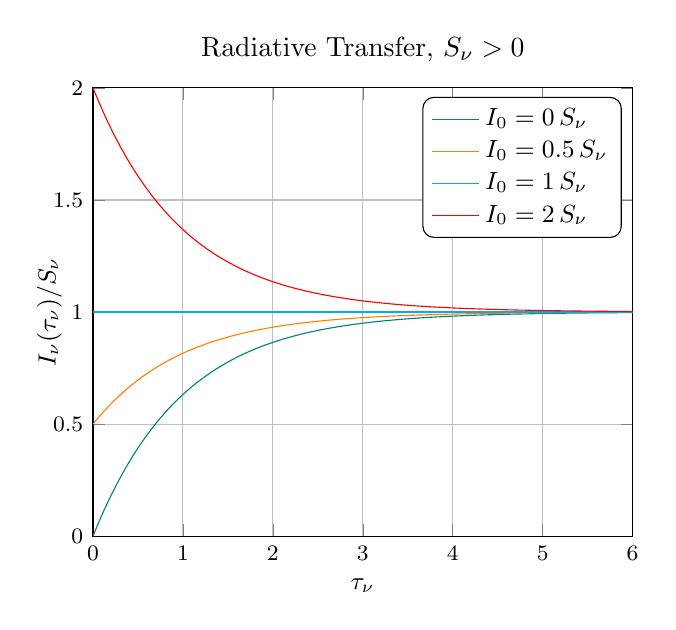
\begin{tikzpicture}

\begin{axis}[%
        xmin=0, xmax=6,
        ymin=0, ymax=2,
        title=Radiative Transfer{,} $S_{\nu}>0$,
        xlabel=$\tau_{\nu}$,
        ylabel=$I_{\nu}(\tau_{\nu})/S_{\nu}$,
        ylabel style={yshift=-1em},
        label style={font=\small},
        tick label style={font=\footnotesize},
        grid=major,
        legend cell align=left,
        legend style={rounded corners,font=\small},
        domain=0:6,
        samples=100,
        cycle list={%
            teal,
            orange,
            cyan,
            red
        },
    ]
    \foreach \I in {0, 0.5, 1, 2}{%
        \addplot {\I*exp(-x)-exp(-x)+1};
        \addlegendentryexpanded{$I_0=\I\,S_{\nu}$}
    };

\end{axis}

\end{tikzpicture}

\end{document}
